\section{Android Apps}\label{sec:sota_apps}
In this section we investigate the state of the art for synchronized streaming of music between different mobile devices.
We found three apps capable this:
\begin{itemize}
    \item SoundSeeder
    \item AmpMe
    \item Chorus
\end{itemize}

These apps are found by searching sources like Google\footnote{https://www.google.dk}, YouTube\footnote{https://www.youtube.com/}, App Store\footnote{https://itunes.apple.com/dk}, and Google Play Store\footnote{https://play.google.com/store} and from recommendations on forums. 
A criteria for an app was that the it must not be depreciated or abandoned by its developers.
The way to estimate this was done by looking at the last update date on Google Play Store and App Store.
For instance if an app had not been updated for a long time, e.g. since 2013 and it do not support new devices, it is probably abandoned.

To clarify, Google Play Store and App Store are the official place to install or buy apps for Android and iOS devices respectively.

The three apps all use a master/slave connection.
All three apps use different terms for their setup, for clarification we generalise these terms. 
We call the device which selects the music and streams it, the master.
The devices which connects to the master (SoundSeeder calls it ``Speaker''), are referred to as slaves.

\subsection{SoundSeeder}\label{subsec:soundseeder}
SoundSeeder\footnote{http://soundseeder.com} is an app made by JekApps. 
The current (and tested) version is 1.6.5.

It is compatible with Android 4.1 and above, for older versions of Android (2.2 -- 4.0),
another app called SoundSeeder Speaker makes it possible for the device to be used as a slave.

SoundSeeder also provides a Java application for compatibility with other platforms e.g. Windows, macOS and Linux.
SoundSeeder does not support iOS and Windows Phone\cite{soundseeder_ios}.

The app consists of a top menu and a burger menu at he left side, as seen on \cref{fig:soundseeder_screenshot}.
In the burger menu, the user can choose the different playback possibilities and switch to slave mode.
The main view of the app is a music player, where the music can be controlled as any other music player. 
To play music to other devices as a master, press the ``add music button'' in the top menu,
choose the source of the music and choose the preferred music, and press play. 

To connect to a playing master device as a slave, select the speaker mode from the burger menu and if it finds the device, it connects automatically.
It took a bit of time before the slave device found the master device, which can seem confusing and make users think they need to connect manually with an IP address. 

The process of joining, when the slave is given the time, is rather simple.
In regard to the user interface, it is clotted with features and menus, which makes the app hard to navigate.
The design of the app is old and not pretty.

SoundSeeder streams music via Wi-Fi or the build--in Android hotspot, 
which means that all phones have to be on the same network\cite{soundseether_faq}.
In regard to the master's music source, it can be Google Music, online radio stations, UPnP and DLNA devices, local media, and YouTube if using semperVidLinks, an app for extracting video links.
SoundSeeder also supports streams from external sources, e.g. a microphone or AUX device. 
The supported media formats depend on the used master device and its Android version.\cite{soundseether_faq}

SoundSeeder synchronizes the music when a slave it connected, but it can also be done manually on the slave device. 
On \cref{fig:soundseeder_slider}, the manual synchronization adjustment for SoundSeeder can be seen.
This slider is used in the case that the music is not fully synchronized, the slider goes from $-100 ms$ up to $+100 ms$.
Furthermore there is also an auto synchronization button in the top menu and on the slider menu window. 

SoundSeeder is free to install but the free version only allows two slave devices to connect for up to 15 minutes at a time.
The full app costs 39.90 DKK. 

\begin{figure}[h!]
    \setlength{\fboxsep}{0pt}
    \setlength{\fboxrule}{2pt}
    \begin{minipage}[b]{0.45\textwidth}
        \centering    
        \fbox{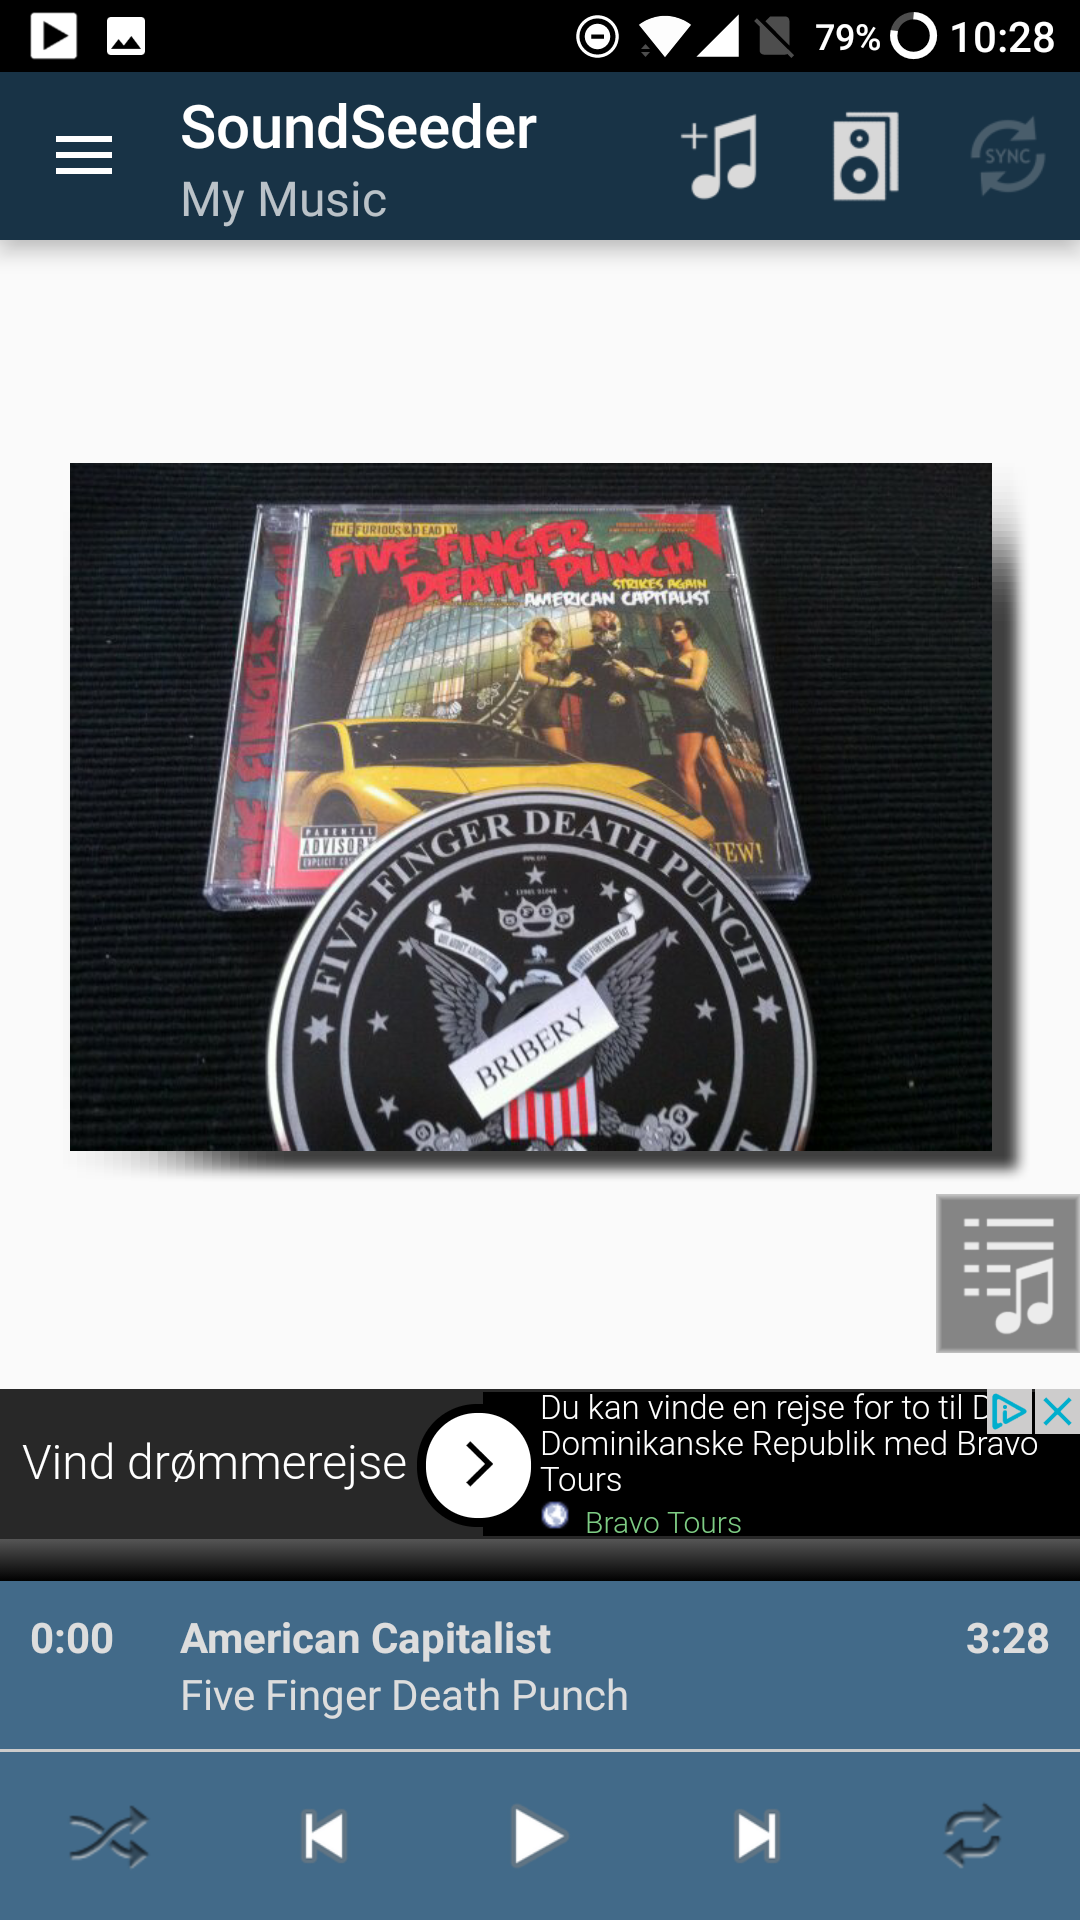
\includegraphics[width=0.65\textwidth]{img/sota/soundseeder.png}}
        \caption{A screenshot of SoundSeeder when the app is opened.}\label{fig:soundseeder_screenshot}
    \end{minipage}
    \hfill
    \begin{minipage}[b]{0.45\textwidth}
        \centering
        \fbox{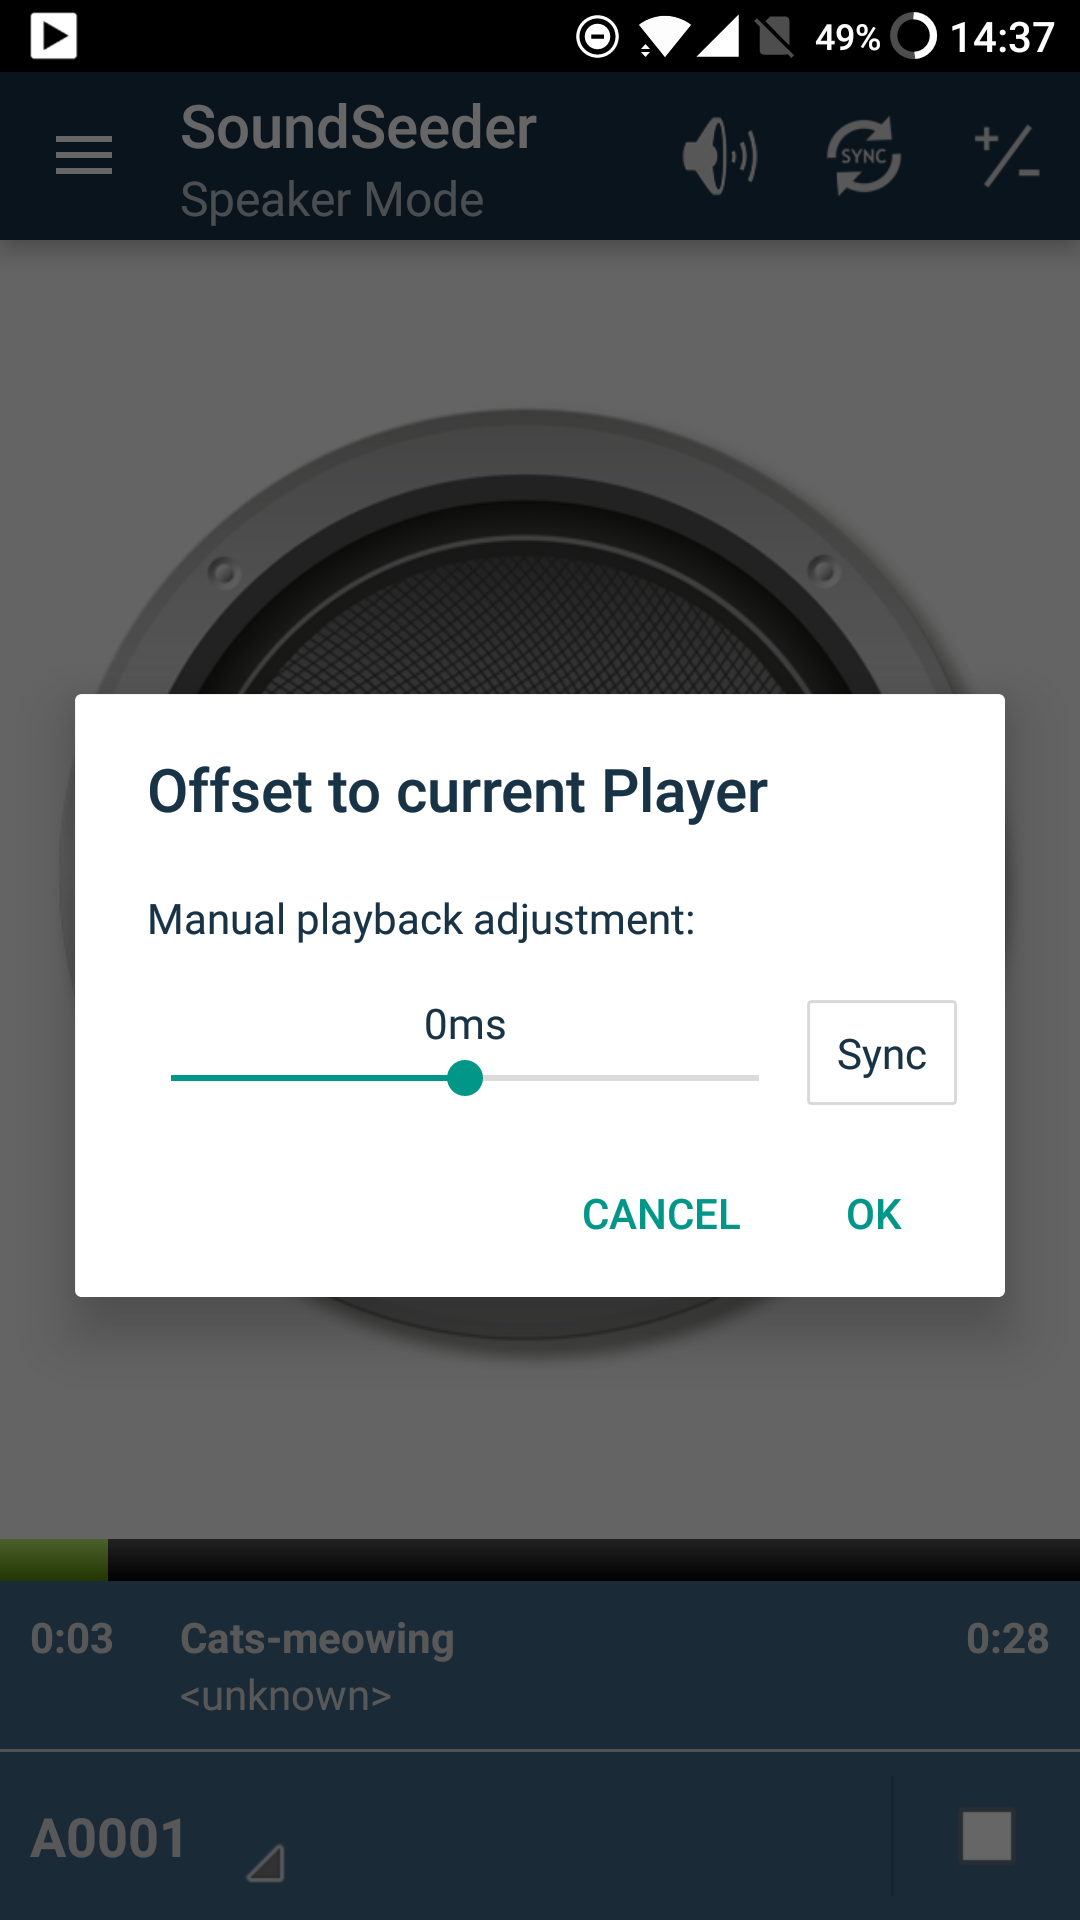
\includegraphics[width=0.65\textwidth]{img/sota/soundseeder_slider.png}}
        \caption{A screenshot of SoundSeeder's synchronization slider.}\label{fig:soundseeder_slider}
    \end{minipage}
\end{figure}

\iffalse
3.9 stars on Google Play
Functionality / How good it works
11. november 2016 https://play.google.com/store/apps/details?id=com.kattwinkel.android.soundseeder.player
For Android > 4.1 and Java based devices (RPI, Linux, Windows, macOS etc.), no plans for iOS and Windows Phone http://soundseeder.com/support/topic/ios-and-windows-support-soon/
Google Music, YouTube (via semperVidLinks app), online radiostations, 
Steam music via Wi-Fi or portable hotspot, UPnP/DLNA browser, mp3, mp4, m4a, aac, 3gp, ogg, flac (depends on your device / android version)
Free version: two speaksers for up to 15 min as often you want, it contains banner adds. Priced version: 39,90 DKK
Sync settings: ?
\fi

\subsection{AmpMe}\label{subsec:ampme}
The second app is AmpMe\footnote{http://www.ampme.com}, made by Amp Me Inc.
It supports Android 4.1 or newer and iOS 9.0 or newer.

In AmpMe the group of devices is called ``a party''.
When AmpMe is opened, it either displays the nearby parties or encourage you to create your own. 
If a party if found, you can join it as a slave and play the master's music.
If no party is found, or you want to create your own, you can choose to start it by choosing between Spotify, 
YouTube, your own music library, or SoundCloud as music source, as shown on \cref{fig:ampme_screenshot}. 
When a source and music is chosen, a player appears with the music playing,
and your device works as a master.

It is very intuitive to join a party, or host one yourself and play music.
Furthermore the interface is modern, minimalistic, and pleasant to use and look at. 

In order to stream music from a master to slaves, AmpMe requires internet, in the form of WiFi or mobile data.
This means that the connected devices can be on WiFi, mobile data or another network, as long there is Internet access. 

In AmpMe, the music is automatically synchronized upon party creation,
but if there is a delay, it can be synchronized manually on the slave.
On \cref{fig:ampme_screenshot} the slider to manually synchronize can be seen.
The slider goes from an offset of $-15$ to $+15$ arbitrary offset units.

AmpMe is free to use in both Google Play and App Store.\cite{amp_faq}\cite{amp_play}\cite{amp_itunes}

\begin{figure}[h!]
\setlength{\fboxsep}{0pt}
    \setlength{\fboxrule}{2pt}
    \begin{minipage}[b]{0.45\textwidth}
        \centering
        \fbox{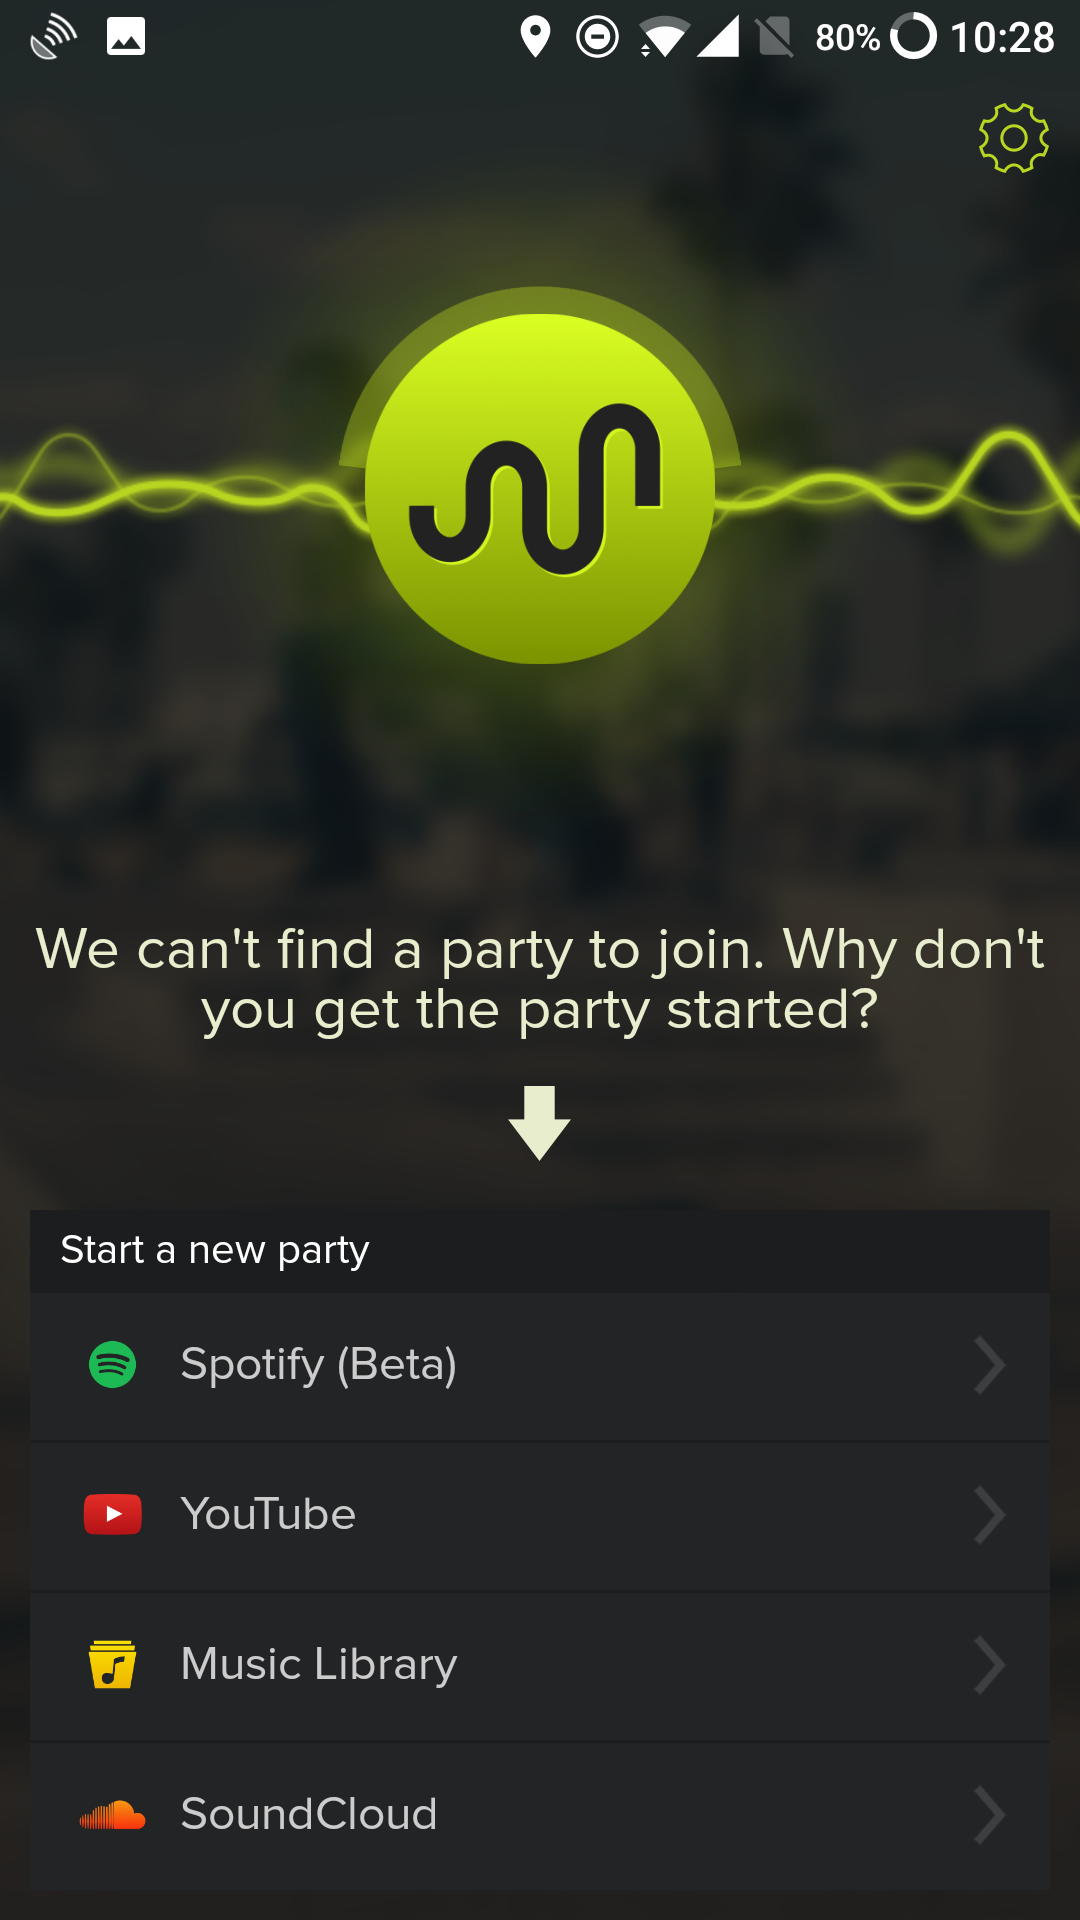
\includegraphics[width=0.65\textwidth]{img/sota/ampme.png}}
        \caption{A screenshot of AmpMe when the app is opened.}\label{fig:ampme_screenshot}
    \end{minipage}
    \hfill
    \begin{minipage}[b]{0.45\textwidth}
        \centering
        \fbox{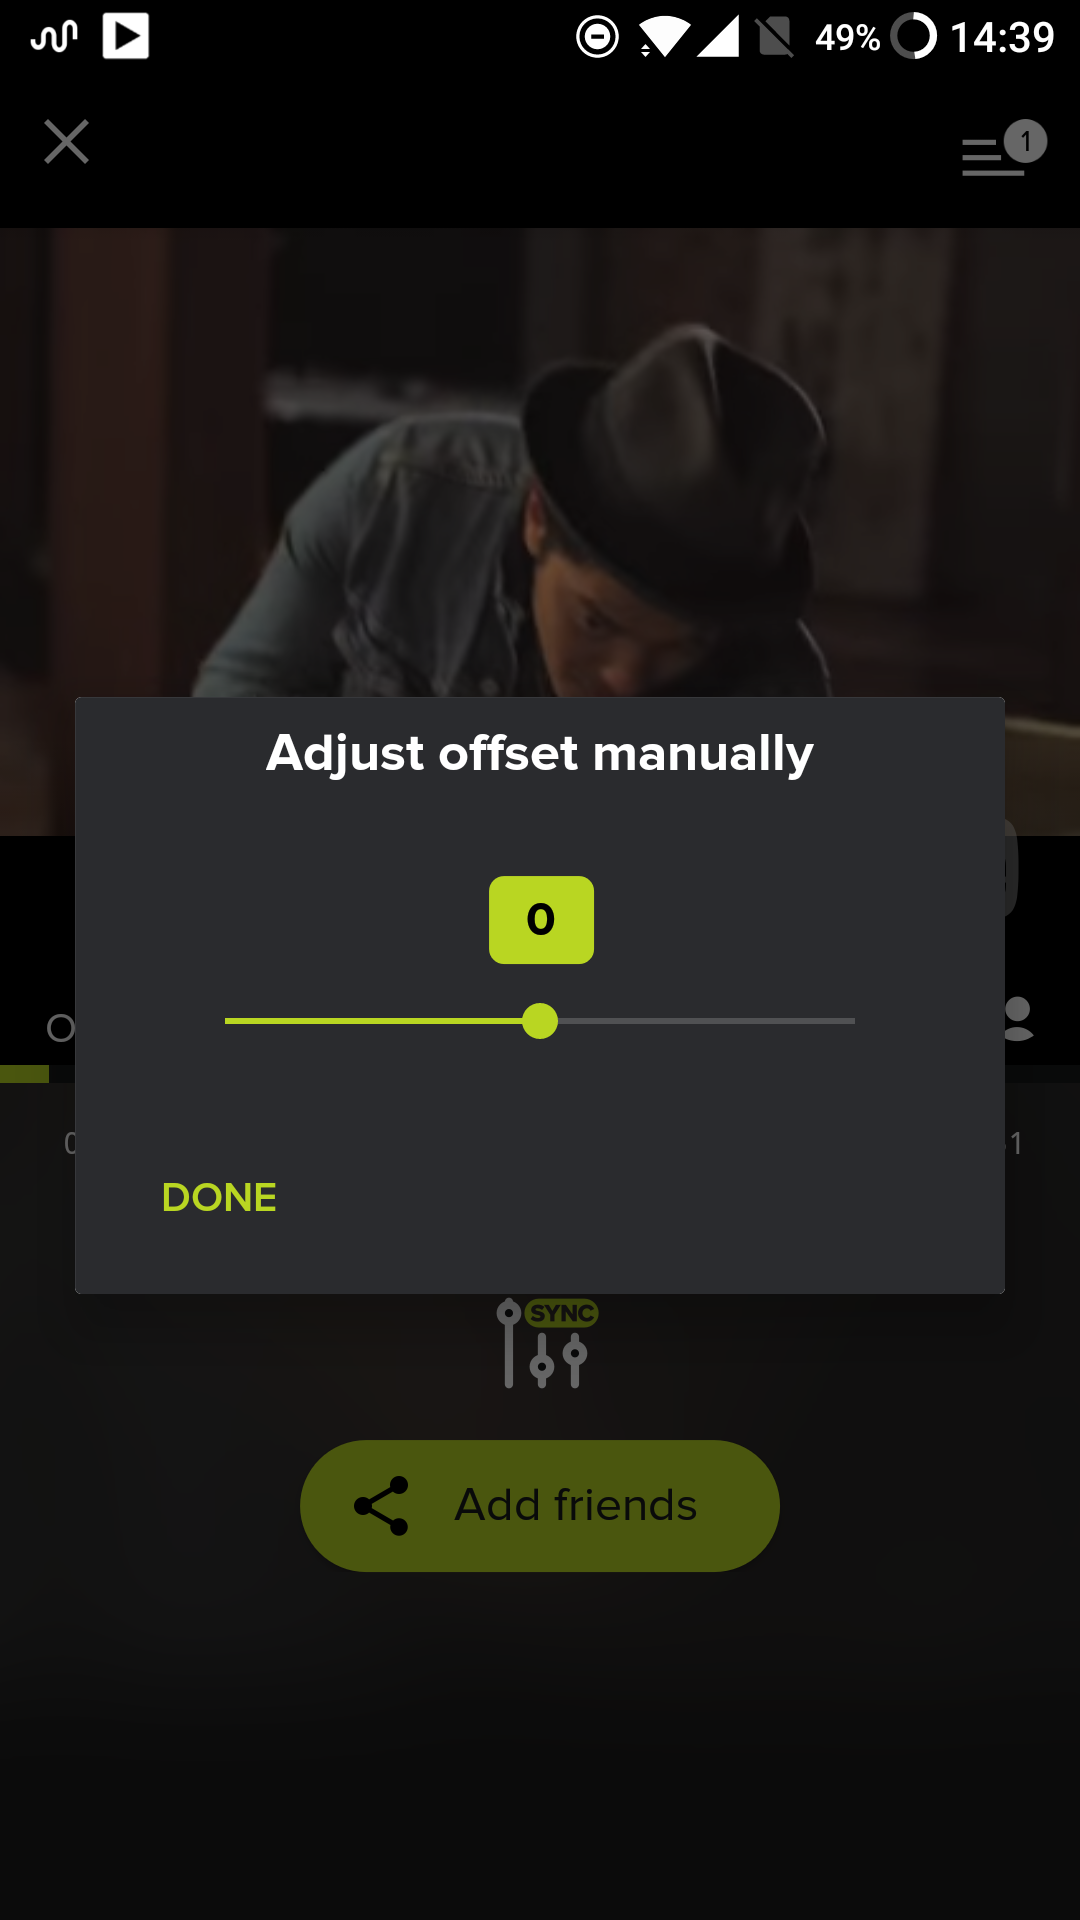
\includegraphics[width=0.65\textwidth]{img/sota/ampme_slider.png}}
        \caption{A screenshot of AmpMe's synchronization slider.}\label{fig:ampme_slider}
    \end{minipage}
\end{figure}

\iffalse
By Amp Me Inc.
4.2 stars on Google Play, current version, 3.5 stars, all versions 4 stars on App Store
Functionality / How good it works
30. januar 2017 (Android), Feb 01, 2017 (iOS)
Android and iOS
Spotify, SoundCloud, YouTube and your local music library
Require internet, WiFi/Mobile data
Free
Resync button, syncs upon connection
\fi

\subsection{Chorus}\label{subsec:chorus}
The final app is called Chorus\footnote{https://play.google.com/store/apps/details?id=com.avrapps.chorus} and is made by AVR APPS.
The used version of the app is 2.1.
It supports Android 4.0 or newer, AVR APPS mention an iOS app, but the App Store page returns that the app is not available in our region,
when open in iTunes\footnote{https://itunes.apple.com/app/chorus/id894014439}.

To share music between devices, WiFi or mobile hotspot is required,
which means that all devices have to be on the same network.
Chorus only supports playback of local media, so the music have to be in memory on the master device.

When the app is opened, it looks like a regular music player, as seen on \cref{fig:chorus_screenshot}.
Music is added by pressing the small plus sign in the right bottom corner. 
When that music is added, Chorus streams the music to connected slave devices.
To connect to a master device playing music, you press the menu button in the right top corner, and press join.
Here a menu pops up with devices playing on the network, and if you select the device shown, it connects as a slave and starts playing.
We encountered a scenario where the app just kept loading when attempting to join an active network, after a restart of the app it worked.

It is intuitive to use the app, it is very minimalistic hence easy to navigate.
The design is a bit old but its simplicity makes up for it.

Chorus supports manual and automatic synchronization.
On \cref{fig:chorus_screenshot} the synchronization slider can be seen,
it slides from $-400ms$ to $+400ms$, and each step is $\Delta 10ms$.

The app is free to download and use without any adds.\cite{chrous_play} 

\begin{figure}[h!]
    \setlength{\fboxsep}{0pt}
    \setlength{\fboxrule}{2pt}
    \begin{minipage}[b]{0.45\textwidth}
        \centering
        \fbox{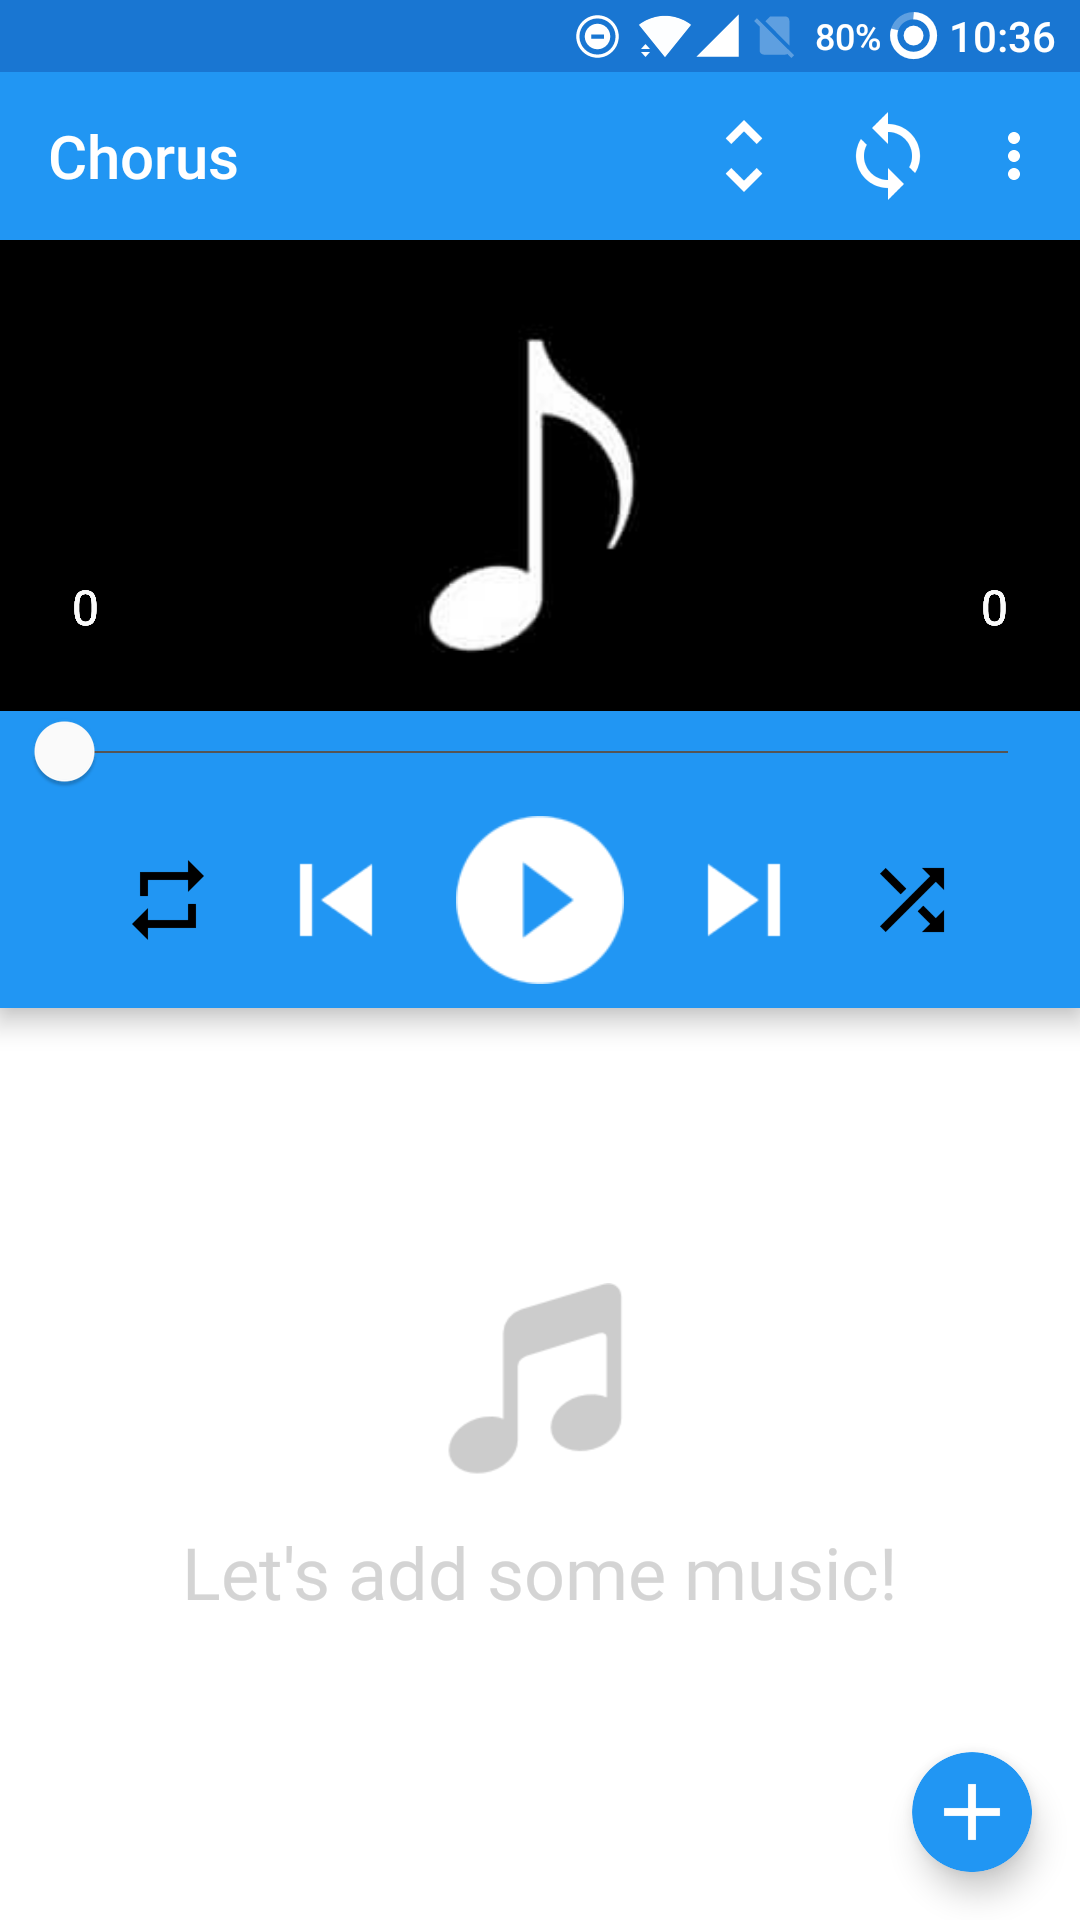
\includegraphics[width=0.65\textwidth]{img/sota/chorus.png}}
        \caption{A screenshot of Chorus when the app is opened.}\label{fig:chorus_screenshot}
    \end{minipage}
    \hfill
    \begin{minipage}[b]{0.45\textwidth}
        \centering
        \fbox{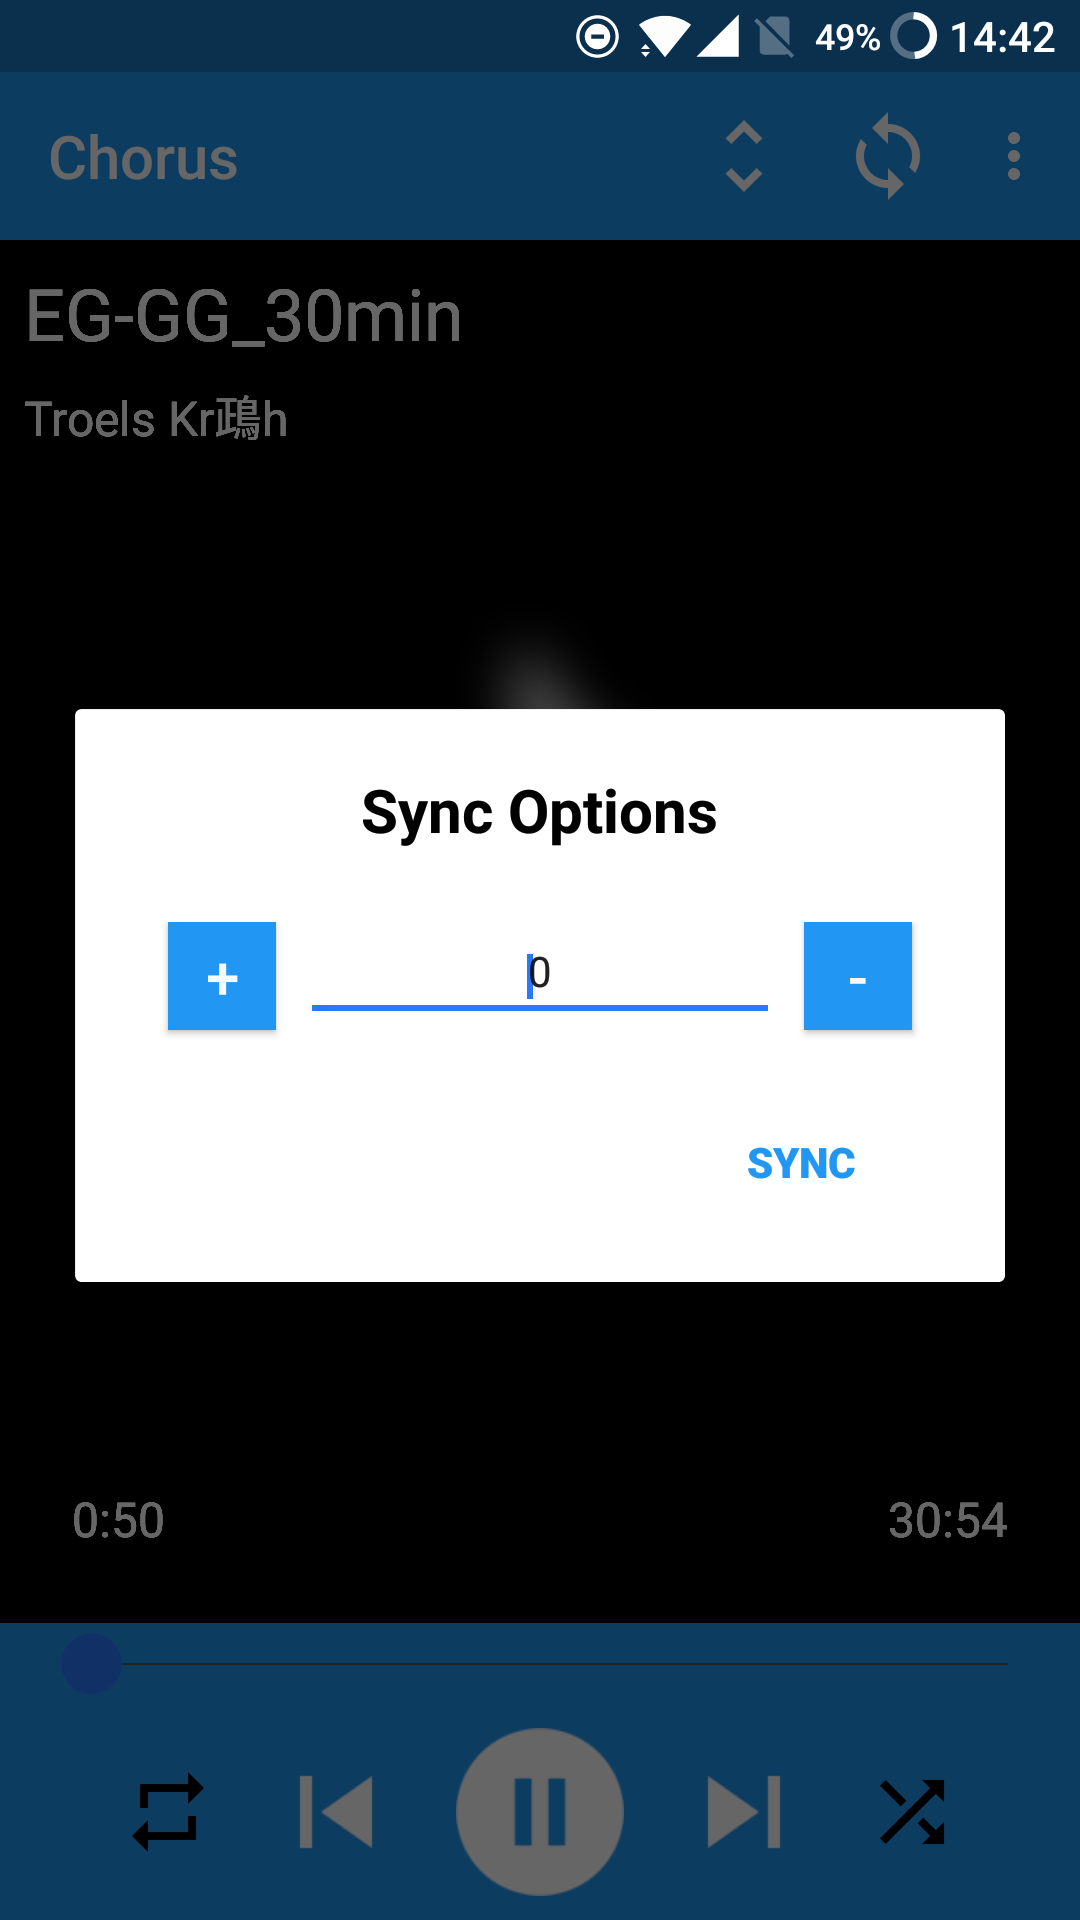
\includegraphics[width=0.65\textwidth]{img/sota/chorus_slider.png}}
        \caption{A screenshot of Chorus' synchronization slider.}\label{fig:chorus_slider}
    \end{minipage}
\end{figure}

\iffalse
By AVR APPS 
3.3 stars on Google Play
Functionality / How good it works
11. maj 2015
Android 4.0, iOS
Local media?
Mobile hotspot or WiFi
Free
Manual/automatic sync
\fi
\subsection{Conclusion}
To determine the state of the art in regard to Android apps, we compare the described apps.
In \cref{tab:sota_comp}, a comparison of the apps can be seen. 

In regard to SoundSeeder versus AmpMe, then in the rating, last update, and supported devices, they are pretty equal.
When it comes to the media source, they both supports YouTube and local media. 
AmpMe supports Spotify, which is very popular, but SoundSeeder supports more different and basic technologies,
like DLNA and UPnP, which makes it possible to e.g. stream from a media server.
SoundSeeder also supports the possibility of using an external device as media source,
which could make it possible to use another device to play Spotity (or SoundCloud for that matter) to the master device,
and then stream it to the connected slaves. 
This could maybe impair the mobility, but that is very dependent on the situation.

On the other hand, AmpMe does not require the devices to be on the same network, only to have an Internet connection,
where SoundSeeder requires the devices to be on the same network.
This can be an annoyance in the case where there is no WiFi available and all devices have to be on the same access point.
Furthermore AmpMe is free to use, where SoundSeeder cost 39.90 DKK for the full version.

When testing the user interface of the two apps in \cref{subsec:soundseeder} and \cref{subsec:ampme}, AmpMe felt more modern and easier to use,
where SoundSeeder is clotted with features.

Looking at Chorus, it is inferior in regard to the rating, last update, and media source.
Especially the media source, where it only supports local media is big downturn. 
The user interface os better than SoundSeeder, but not as good as AmpMe.

To draw a conclusion on the comparison of the apps,
we deem that SoundSeeder and AmpMe represent the state of the art in streaming synchronized music to mobile devices. 
This is because SoundSeeder has a lot of useful features and AmpMe has a very good user interface, Spotify support and is free to use. 
We do not feel that Chorus has enough extra features than just streaming synchronized music to be a part of the state of the art.
Furthermore since Chorus has not been updated since the 11\textsuperscript{th} of May 2015,
it is probably not going to get any new features in the future.

\begin{table}
    \scalebox{0.9}{
    \begin{tabular}{l|l|l|p{2.2cm}|p{2.5cm}|p{2.4cm}|p{2.0cm}|}
                    & \multirow{2}{*}{Rating}    & \multirow{2}{*}{Last update}   & Supported devices & \multirow{2}{*}{Media source} & \multirow{2}{*}{Connectivity} & \multirow{2}{*}{Pricing}  \\
        \toprule

        \multirow{7}{*}{SoundSeeder} & \multirow{7}{*}{3.9 Play Store}    & \multirow{7}{*}{11/11 2016}    & \multirow{6}{*}{Android 4.1$\le$,} & Google Music, & \multirow{6}{*}{WiFi,} &  \multirow{6}{*}{Free (limited),} \\
    & & & \multirow{6}{*}{Java devices} & YouTube, & \multirow{6}{*}{Android hotspot} & \multirow{6}{*}{39.90 DKK} \\
    & & & & external device, & & \\
    & & & & UPnP, & & \\
    & & & & DLNA, & & \\
    & & & & online radio, & & \\
    & & & & local media & & \\ 

    \midrule

        \multirow{4}{*}{AmpMe} & \multirow{3}{*}{4.2 Play Store} & \multirow{3}{*}{30/01 2017} & \multirow{3}{*}{Android 4.1$\le$,} & Spotify, & \multirow{4}{*}{Internet} & \multirow{4}{*}{Free} \\
    & \multirow{3}{*}{4.0 App Store} & \multirow{3}{*}{01/02 2017} & \multirow{3}{*}{iOS 9.0 $\le$} & SoundCloud, & & \\
    & & & & YouTube, & & \\
    & & & & local media & & \\

    \midrule

        \multirow{2}{*}{Chorus} & \multirow{2}{*}{3.3 Play Store} & \multirow{2}{*}{11/5 2015} & \multirow{2}{*}{Android 4.0 $\le$} & \multirow{2}{*}{Local media} & \multirow{1}{*}{WiFi,} & \multirow{2}{*}{Free} \\
    & & & & & \multirow{1}{*}{Android hotspot} & \\

    \bottomrule

    \end{tabular}}
    \caption{Comparison between the apps.}\label{tab:sota_comp}
\end{table}



%Savner generelt en vinkel som er brugbar for os. Der er fokus på user experience hvilket vi ikke rigtig kan bruge til noget i vores project, dette gælder også de enkelte paragrapher der er rundt omkring omkring minimalistisk og simplistisk design. - Conclusionen virker for mig som et app-review du finder på buzzfeed for at finde ud af hvilken app du skal vælge, from for at udmunde i noget som vi kan gå videre med i vores project

%Synes det burde være mere analyse, mindre review - ved godt det er seperat fra tests men synes stadig der burde være value i afsnittet, et eksempel ville være at overveje hvorfor har alle en manual synch feature, hvordan affecter det vores sync, bruger de mic til at autosynch? hvordan virker deres autosynch features hvis du kan finde noget om det - mere dybdegående information kan godt findes uden test
